\documentclass[tikz,border=10pt]{standalone}
\usepackage{tikz}
\begin{document}
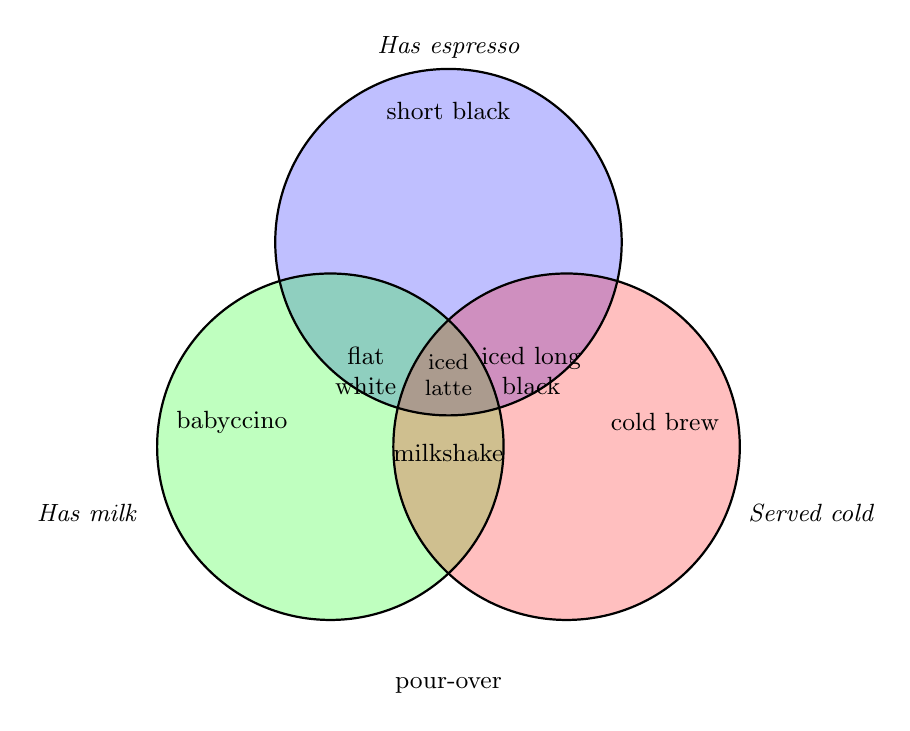
\begin{tikzpicture}[font=\small]
  \def\r{2.2}
  \def\e{(0,1.732)}      % Has espresso
  \def\m{(-1.5,-0.866)}  % Has milk
  \def\c{(1.5,-0.866)}   % Served cold

  \begin{scope}[fill opacity=0.25, text opacity=1]
    \fill[blue]  \e circle (\r);
    \fill[green] \m circle (\r);
    \fill[red]   \c circle (\r);
  \end{scope}
  \draw[thick] \e circle (\r);
  \draw[thick] \m circle (\r);
  \draw[thick] \c circle (\r);

  % circle titles
  \node[font=\small\itshape] at (0,4.2)      {Has espresso};
  \node[font=\small\itshape] at (-4.6,-1.7)  {Has milk};
  \node[font=\small\itshape] at (4.6,-1.7)   {Served cold};

  % outside all three
  \node at (0,-3.9) {pour-over};

  % single regions
  \node at (0,3.4)     {short black};
  \node at (-2.75,-0.55) {babyccino};
  \node at (2.75,-0.55)  {cold brew};

  % pairwise regions
  \node[align=center] at (-1.05,0.1)  {flat\\white};
  \node[align=center] at (1.05,0.1)   {iced long\\black};
  \node at (0,-0.95)                  {milkshake};

  % triple region
  \node[align=center,font=\footnotesize] at (0,0.05) {iced\\latte};
\end{tikzpicture}
\end{document}
